\documentclass[10pt,letterpaper]{article}
\usepackage[top=0.85in,left=2.75in,footskip=0.75in,marginparwidth=2in]{geometry}

% use Unicode characters - try changing the option if you run into troubles with special characters (e.g. umlauts)
\usepackage[utf8]{inputenc}

% clean citations
\usepackage{cite}

% hyperref makes references clicky. use \url{www.example.com} or \href{www.example.com}{description} to add a clicky url
\usepackage{nameref,hyperref}

% line numbers
\usepackage[right]{lineno}

% improves typesetting in LaTeX
\usepackage{microtype}
\DisableLigatures[f]{encoding = *, family = * }

% text layout - change as needed
\raggedright
\setlength{\parindent}{0.5cm}
\textwidth 5.25in 
\textheight 8.75in

% use adjustwidth environment to exceed text width (see examples in text)
\usepackage{changepage}

% adjust caption style
\usepackage[aboveskip=1pt,labelfont=bf,labelsep=period,singlelinecheck=off]{caption}

% remove brackets from references
\makeatletter
\renewcommand{\@biblabel}[1]{\quad#1.}
\makeatother

% headrule, footrule and page numbers
\usepackage{lastpage,fancyhdr,graphicx}
\usepackage{epstopdf}
\pagestyle{myheadings}
\pagestyle{fancy}
\fancyhf{}
\rfoot{\thepage/\pageref{LastPage}}
\renewcommand{\footrule}{\hrule height 2pt \vspace{2mm}}
\fancyheadoffset[L]{2.25in}
\fancyfootoffset[L]{2.25in}

% use \textcolor{color}{text} for colored text (e.g. highlight to-do areas)
\usepackage{color}

% define custom colors (this one is for figure captions)
\definecolor{Gray}{gray}{.25}

% this is required to include graphics
\usepackage{graphicx}

% use if you want to put caption to the side of the figure - see example in text
\usepackage{sidecap}

% use for have text wrap around figures
\usepackage{wrapfig}
\usepackage[pscoord]{eso-pic}
\usepackage[fulladjust]{marginnote}
\reversemarginpar

% document begins here
\begin{document}
\vspace*{0.35in}

\title{Network visualizations in reproducible workflows using Jupyter}

% title goes here:
\begin{flushleft}
{\Large
\textbf\newline{Network visualizations in reproducible workflows using Jupyter}
}
\newline
% authors go here:
\\
Author 1\textsuperscript{1},
Author 2\textsuperscript{2},
Author 3\textsuperscript{1},
Author 4\textsuperscript{1},
Author 5\textsuperscript{2},
Author 6\textsuperscript{2},
Author 7\textsuperscript{1,*}
\\
\bigskip
\bf{1} Affiliation A
\\
\bf{2} Affiliation B
\\
\bigskip
* correseponding@author.mail

\end{flushleft}

% now start line numbers
\linenumbers

%%%%%%%%%%%%%%%%%%%%%%%%% paste begin

% ---------------------------------------------------------------------
% EG author guidelines plus sample file for EG publication using LaTeX2e input
% D.Fellner, v1.17, Sep 23, 2010

%\title{Network visualizations in reproducible workflows using Jupyter}

% for anonymous conference submission please enter your SUBMISSION ID
% instead of the author's name (and leave the affiliation blank) !!
%\author[A. Watters]
%       {A.\,R. Watters$^{1}$
%        \\
% For Computer Graphics Forum: Please use the abbreviation of your first name.
%         $^1$Center for Computation Biology, Flatiron Institute of the Simons Foundation
%       }

%\author[EuroVis 2017 Short Papers Submission 176] {
%  EuroVis 2017 Short Papers Submission 176
%}

% ------------------------------------------------------------------------

% if the Editors-in-Chief have given you the data, you may uncomment
% the following five lines and insert it here
%
% \volume{27}   % the volume in which the issue will be published;
% \issue{1}     % the issue number of the publication
% \pStartPage{1}      % set starting page


%-------------------------------------------------------------------------
%\begin{document}

% \teaser{
%  \includegraphics[width=\linewidth]{eg_new}
%  \centering
%   \caption{New EG Logo}
% \label{teaser}
% }

\maketitle

\section*{Abstract}
%\begin{abstract}
Transcriptional regulatory networks (TRNs) 
describe how gene expression is regulated in diverse cell types, tissues, and
organisms in response to environmental cues.    
We describe a methodology for sharing 
executable workflows for deriving, comparing,  and analysing TRNs and 
related gene expression data.  
The methodology uses archives orchestrated 
by Jupyter notebook narrative documents and allows for seamless integration
of visualizations with R and Python programs used to derive TRNs and process
genomics data.  
These documents include key 
interactive visualization tools designed to help researchers explore and 
understand TRNs and the relationship of TRNs to gene expression matrices 
and other data.  The workflows run on any platform in standard web browsers.

%\begin{classification} % according to http://www.acm.org/class/1998/
%\CCScat{Computer Graphics}{I.3.4}{Graphics Utilities}{Graphics editors}
%\CCScat{Database Management}{H.2.8}{Database Applications}{Data mining}
%\end{classification}

%\end{abstract}


%%%
%%% Figure Linked
%%%
\begin{figure}[htb]
  \centering
  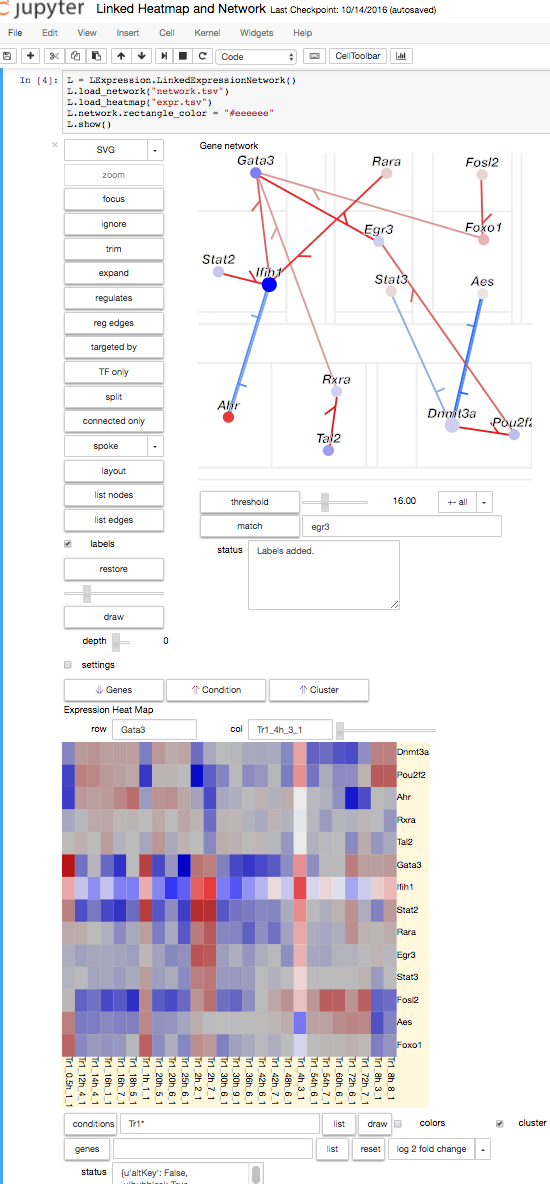
\includegraphics[width=.6\linewidth]{Linked}
  \caption{\label{Linked}
           An interactive heatmap of gene expression data (below) linked to a TRN network model visualization (above).  
           Genes of the network have been clustered by similar expression pattern in the heatmap and 
           are restricted to transcription factors related to the EGR3 gene.  Expression levels in the heatmap 
           are normalized by log 2 fold change and are restricted to 
           the genes of the network under the experimental conditions matching “Tr1*”.  Nodes of the network
           are colorized by expression levels in the experimental condition "Tr1\_4h\_3\_1".
  }
\end{figure}

%%%
%%% Figure motif
%%%
\begin{figure}[htb]
  \centering
  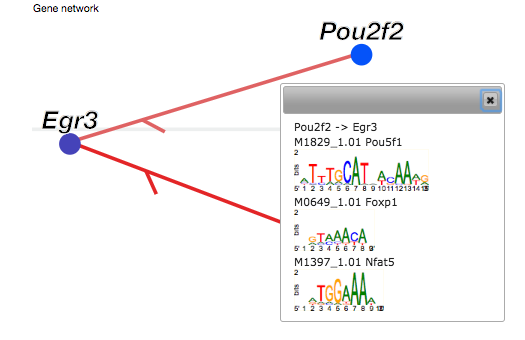
\includegraphics[width=.8\linewidth]{motif}
  \caption{\label{motif}
           A network annotated with sequence motifs displays the motifs associated with a transcriptional 
           relationship on mousing over the edge for the association.
  }
\end{figure}

%%%
%%% Figure pair
%%%
\begin{figure}[htb]
  \centering
  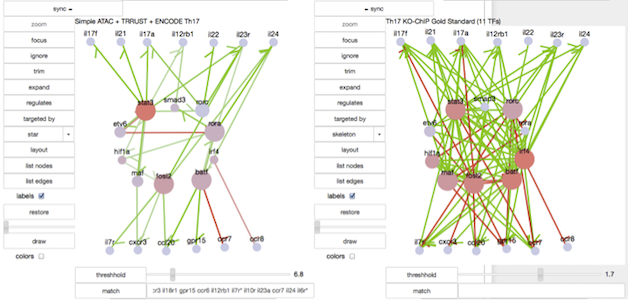
\includegraphics[width=.8\linewidth]{pair}
  \caption{\label{pair}
           A multiple network display comparing a “core” TRN (right) with an inferred TRN (left).  
           The multiple network view coordinates any number of networks arranged in a rectangular array.
  }
\end{figure}



%-------------------------------------------------------------------------
\section{Introduction}

Many experimental designs today aim to derive network models of regulation of 
gene transcription \cite{arrieta2015, Blatti2015, yosef2013, karwacz2017} from 
high throughput transcriptomic sequencing data \cite{reuter2015} and 
other genomics technologies or data sources.  
These studies frequently involve several researchers working in different locations 
who have different expertise, from experimental methods to computational 
inference of TRNs \cite{inferelator, wang2006}. 

This  paper describes a methodology for documenting the derivation, analysis, 
and visualization of TRNs and for comparing TRNs to gene expression data and 
other evidence using repositories containing Jupyter notebook documents 
\cite{ipython} and other source files.  These workflows include widgets that implement 
interactive visualizations designed to present and explore TRNs, implemented in 
the {\em jp\_gene\_viz} project \cite{jpgeneviz}. All notebook interactions including interactive 
visualizations can be completely automated by the notebook author using simple 
script fragments allowing other researchers such as collaborators, reviewers, 
or auditors to reproduce all research results.  The notebooks of the archive 
can be executed by researchers remotely using cloud web services such as {\em binder} \cite{binder} 
without the need to install any special purpose software on the local machine.

\section{Related Work}

There are many tools for visualizing TRNs \cite{VizBi} including 
stand alone applications \cite{Partl, cytoscape, gephi} 
and special purpose web applications \cite{genotet}.  
Other general network visualization tools use sophisticated query 
models to help users explore network models in many domains \cite{Kairam15}.

This work presents an alternative visualization methodology 
which is designed to be used in Jupyter based workflows.  
This paper focusses on the visualization widgets in {\em jp\_gene\_viz} specifically designed to present 
and explore TRNs and we limit our attention to Jupyter notebooks
driven by the R and Python Jupyter kernels.
The interactions provided by the widgets we describe include 
dozens of operations requested by researchers interested in 
deriving and analysing TRNs and related data.  
Notebook narratives may include preprocessing for the upstream inputs 
to the visualization widgets and may extract the results derived 
from visualization transformations and use those outputs in
 downstream processing.  These network visualizations inputs and outputs 
 may be freely combined with other components of the Jupyter 
 ecosystem such as statistical classification tools 
 provided by scikit-learn \cite{scikit-learn} and other 
 mathematical tools provided by SciPy \cite{scipy} for Python based
 notebooks, or the Bioconductor packages for R based notebooks \cite{bioconductor}.
 The outputs may also be 
 fed to subprocesses controlled from the Jupyter notebook document.  

Other visualizations can be used in combination with the jp\_gene\_viz 
widgets to present the data in alternate ways in the Jupyter environment 
such as the matplotlib plotting library \cite{matplotlib} and any 
Javascript based HTML5 library such as the Cytoscape.js \cite{cytoscapejs} 
network display library or the Highcharts chart libraries \cite{highcharts}.

\section{Building reproducible workflow archives with interactive visualizations}

Workflow archives include source data and computations for generating output 
data as well as visualizations or other derivative products.  The archives 
should explain the operation and justifications for each step of the workflow.
These requirements are easily implemented using folders containing Jupyter 
notebooks and required data files.

Jupyter notebooks consist of a sequence of documentation cells and executable cells
followed by static text or visualization results or by interactive widget visualizations.
Executable notebook cells
support general purpose computation using Python or R script fragments, 
subprocesses, and shell command lines.  A workflow should organize all high level 
operations as a sequence of notebooks which perform all operations of the workflow 
and include discussion text explaining each step of the workflow formatted using 
documentation cells.  An “index” notebook should provide an entry point with 
introductory information and links to the other notebooks of the workflow.  
The actions of each notebooks should be idempotent in the sense the notebook 
produces the same output artifacts whenever it is executed with the same inputs 
unless the notebook is modified by the user in some manner.

To construct a workflow archive a researcher assembles required input files into 
an archive folder and then constructs notebooks for generating outputs from the 
inputs as well as any visualizations.  

Visualizations are typically constructed initially 
in an interactive manner by direct manipulation of interactive
controls which are later emulated using script fragments to make the visualization
reproducible. For example a slider adjusted to level 10 followed
by a  button press can be emulated using the script fragment
\texttt{network.threshold\_slider.value=10; network.expand\_button.click())}.

Once the researcher has captured the workflow process as a sequence of executable notebook 
narratives, with visualization configuration hardened into code cell script fragments, 
the archive must be packaged for distribution.  We capture all software dependencies 
for a workflow by building a Dockerfile designed to build a Docker container \cite{docker} 
that will run the workflow archive in the Binder cloud web service \cite{binder} to
allow collaborators to recreate the software infrastructure for the workflows.  The Dockerfile 
usually uses other configuration files in the build process.

To publish the workflow archive we create a public Github project including all data 
and executable notebooks and any other dependencies.  In some cases we add encryption/decryption 
to the workflow to prevent releasing data which is not appropriate for 
release to unauthorized parties.  At this point we usually build the Github repository 
in the the Binder service \cite{binder} to make the archive available easily to other 
researchers without the need to install software and also to test that the Dockerfile captures all dependencies.  
We then share the location of the Github repository for the workflow and a hyperlink 
for running the archive in Binder with collaborators and other researchers. 

\section{The network visualization components}

The jp\_gene\_viz package includes several interactive Jupyter widgets 
for visualizing and manipulating TRN data and relate gene expression matrices.  
It is not possible to discuss all of the features of these widgets in this short paper -- 
please see the package documentation for further details.  All of these widgets accept and generate 
standard data formats as inputs and outputs.
The programming interface to the widgets may be used to implement interfaces
to other formats and data sources using Jupyter cell script fragments.

The TRN Network interactive visualization is illustrated in the top part of Figure~\ref{Linked}. 
The network consists of a directed weighted graph between nodes labeled with gene names 
and make contain thousands of nodes and edges.  An edge of the graph connects a transcription 
factor gene (TF) with a gene influenced by that factor where a positive weight (shown in shades of red) 
indicates that the TF promotes gene transcription of the target gene or a negative weight (shown in shades of blue)
indicates the TF inhibits transcription of the gene. Nodes and edges of the graph may also be
associated with other information such as node weights and edge binding motifs.  Usually the 
visualization displays a subset of the nodes and edges of the network and many of the 
interactive controls allow the researcher to select the subset of interest and adjust the way 
the subset is presented.  This widget includes dozens of interactive features not described here 
including a hidden panel which allows network display configurations to be exported to various 
formats for publication and archived.  For example, a network can be annotated with sequence motifs 
\cite{motif} associated with transcriptional relationships as illustrated in Figure~\ref{motif}.  
The network widget also supports interactive features for dragging/dropping subsets of the network
to improve layout as well as customization of colors and label sizes.  These features 
were requested by genomics researchers using the widget in workflows.

A TRN network visualization may be linked with a heatmap showing gene expression 
levels under different experimental conditions as shown in Figure~\ref{Linked}.  
The heatmap shows values for each gene as rows and values for each experimental condition as columns.  
There are a number of controls for selecting genes and conditions in the heatmap, for transforming expression 
level values and colorations, and for clustering values by similar expression patterns.
Buttons connect the network visualization to the heatmap.  For example the “Cluster” button uses the expression 
levels shown in the heatmap to group genes of the network with similar expression levels close together.

Any number of TRN networks and linked TRN networks can also be arranged into coordinated 
“multiple network” rectangular array to allow easy comparison of network models.  
Controls allow the researcher to coordinate the network layout of the networks, show differences 
between the networks, and show commonality among the networks.  
Researchers use the multiple network visualization to compare models derived using 
different inference methods, or derived from different experimental conditions.  
Figure~\ref{pair} shows a multiple network view with two coordinated networks.

Researchers use these visualizations in Jupyter notebooks to interactively explore data sets and later often
add script fragments to the notebooks which reproduce specific configurations for the visualizations.
The configuration script fragments may consist of simple assignments or they may be quite sophisticated.  For example
some script fragments read gene lists from external data sources and use those lists to configure
networks and heatmaps.  The Jupyter notebook environment supports novice level programming interactions
and expert level interactions equally well, with a smooth learning curve between the two extremes.

\section{Conclusion}

Genomic technologies used in systems biology evolve rapidly and transcriptomic research
efforts often involve many researchers at different locations with different areas of expertise, from specialists
in laboratory methods, to specialists in statistical analysis, to specialists in
software engineering.  Repositories organized using collections of
Jupyter notebooks allow research teams to share reproducible workflows 
specifying research methods and results.  Programmable
interactive visualization widgets integrated into the workflows allow researchers
to explore data and data relationships and communicate observations to collaborators.

%%%%%%%%%%%%%%%%%%%%%%%%% paste end

\nolinenumbers

%This is where your bibliography is generated. Make sure that your .bib file is actually called library.bib
\bibliography{jp_gene_viz}

%This defines the bibliographies style. Search online for a list of available styles.
\bibliographystyle{abbrv}

\end{document}

